\documentclass[11pt,a4paper,twoside]{report}

% Mathematics
\usepackage{amsmath, amsfonts, mathtools, amsthm, amssymb}
\usepackage{mathrsfs}
\usepackage{cancel}

% Colours
\usepackage[usenames,dvipsnames]{xcolor}
  \definecolor{col1}{HTML}{3A86FF}
  \definecolor{col2}{HTML}{0BBF7D}
  \definecolor{col3}{HTML}{FFBE0B}
  \definecolor{col4}{HTML}{FF006E}
  \definecolor{col5}{HTML}{733907}

% Fonts
\usepackage{libertine}
\usepackage{newtxmath}
\usepackage{fontspec}
\setmonofont[Scale=MatchLowercase]{Courier New Bold}

% Formatting
\usepackage{enumitem}
\usepackage{marginnote}
\usepackage[top=2.5cm,bottom=2.5cm,inner=3.5cm,outer=3cm,marginparwidth=1.5cm]{geometry}
\usepackage{hyperref}
\usepackage{titlesec}
\setlength\parindent{0pt}

% Graphics
\usepackage{graphicx}
\graphicspath{{graphics/}}

% Honestly don't remember
\usepackage[normalem]{ulem}
\usepackage[misc]{ifsym}

% Chapter and section formatting
\titleformat{name=\chapter}[display]{\bfseries\LARGE\itshape\sffamily}{}{0.5ex}{\vspace{1ex}\rule{\textwidth}{1pt}\newline\thechapter.\quad\vspace{1ex}}[\vspace{-0.5ex}\rule{\textwidth}{0.3pt}]

\titleformat{name=\chapter, numberless}[block]{\normalfont\bfseries\LARGE}{}{0em}{}

\titleformat{name=\section, numberless}[display]{\bfseries\sffamily}{}{.5ex}{\thesection~}[\vspace{-0.5ex}%
\rule{\textwidth}{0.3pt}]
% Grid Background
%%%`\GridOn' to enable on page.

\usepackage[pages=some]{background}
\newcommand{\GridOn}{\BgThispage}
\def\Step{5mm}
\backgroundsetup{
scale=1,
angle=0,
contents={
\begin{tikzpicture}[remember picture,overlay]
\draw[step=\Step,help lines,dashed]
  (current page.north west) grid  (current page.south east);
\draw[step=2*\Step,help lines]
  (current page.north west) grid  (current page.south east);
  \end{tikzpicture}
  }
}

% Cloze
%%% `\ShowClozetrue' to enable, `\ShowClozefalse' to disable
\newif\ifShowCloze
\ShowClozefalse
\newcommand{\Cloze}[1]{
    \ifShowCloze
        \dotuline{\parbox[b]{\widthof{\LARGE\textbf{#1}}}{ \vphantom{\vspace{1ex}} \centering %
        {\color{OrangeRed}  {\protect #1}} %
        }}
    \else
        \dotuline{\parbox[b]{\widthof{\LARGE\textbf{#1}}}{ \vphantom{\vspace{1ex}}\centering %
            \hfill
            }
        }
    \fi
}

% Boxes
\usepackage[most]{tcolorbox} % Required for boxes
	\tcbuselibrary{skins,breakable,xparse}
\usepackage{varwidth}

\newtcolorbox[auto counter]{definition}[1][]{standard jigsaw,enhanced,sharp corners,frame hidden,boxrule=0pt,breakable,colback=col1!20!white,fonttitle=\bfseries,coltitle=col1!50!black,colframe=col1!50!white,title=Definition~\thetcbcounter\quad#1\newline,attach title to upper,borderline west={2pt}{0pt}{col1!80!black},left=3mm}

\newtcolorbox[auto counter]{examplebox}[1][]{standard jigsaw,enhanced,sharp corners,frame hidden,boxrule=0pt,breakable,colback=col2!20!white,fonttitle=\bfseries,coltitle=col2!50!black,colframe=col2!50!white,title=Example~\thetcbcounter\quad#1\newline,attach title to upper,borderline west={2pt}{0pt}{col2!80!black},left=3mm,borderline south={1pt}{0pt}{col2!80!black}}

\newtcolorbox{solutionbox}[1][height=4cm]{standard jigsaw,enhanced,sharp corners,frame hidden,boxrule=0pt,breakable,#1,colback=col2!50!white,fonttitle=\bfseries,coltitle=col2!50!black,colframe=col2!50!white,opacityback=.1,title=Solution\newline,attach title to upper,borderline west={2pt}{0pt}{col2!80!black},left=3mm,top=3mm,before={\vspace{-1em}}}

\newtcolorbox{note}{standard jigsaw,enhanced,sharp corners,frame hidden,boxrule=0pt,breakable,colback=col3!20!white,fonttitle=\normalfont\bfseries,coltitle=col3!50!black,colframe=col3!50!white,title=Note~,attach title to upper,borderline west={2pt}{0pt}{col3!80!black},left=3mm,fontupper=\itshape}

\newtcolorbox{important}{standard jigsaw,enhanced,sharp corners,frame hidden,boxrule=0pt,breakable,colback=col4!20!white,fonttitle=\bfseries,coltitle=col4!50!black,colframe=col4!50!white,title=Important note\newline,attach title to upper,borderline west={2pt}{0pt}{col4!80!black},left=3mm}

\newtcolorbox{further}{standard jigsaw,enhanced,sharp corners,frame hidden,boxrule=0pt,breakable,colback=col5!20!white,fonttitle=\bfseries,coltitle=col5!50!black,colframe=col5!50!white,title=Further exercises\newline,attach title to upper,borderline west={2pt}{0pt}{col5!80!black},left=3mm}

\usepackage{environ}

\NewEnviron{example}[2][height=4cm]{
  \begin{examplebox}[#2]
  \BODY
  \end{examplebox}
  \begin{solutionbox}[#1]
  \end{solutionbox}
}

%\usepackage{showframe}

\begin{document}

\ShowClozetrue

\tableofcontents

\chapter{Using the template}

\section{Compiling}

\begin{important}
You'll need to use lualatex\marginnote{xelatex will probably work too!} when you're compiling unless you take out the font changes under \textit{include/structure.tex}
\end{important}

\section{Boxes}

The template has 6 different boxes you can use:
\begin{itemize}
  \item Definition
  \item Example*
  \item \textit{Solution}*%\marginnote{*Are paired together, but can be used separately.}
  \item Note
  \item Important note
  \item Further exercises
\end{itemize}
The definition and example boxes are numbered and can have titled added.

\subsection{Definition box}

\begin{definition}[Title]
  Definition here
\end{definition}

\begin{definition}
  Definition here
\end{definition}

\subsection{Example and solution boxes}

\begin{example}{Title}
  Example here
\end{example}

\begin{example}{}
  Example here
\end{example}

%By default the solution box has a height of 4 cm, but it can be changed by including `[height=?cm]' where ? is replaced with a value. e.g.

\begin{example}[height=2.5cm]{Title}
  Example here
\end{example}

The solution and example boxes can also be made separely by using `examplebox' and `solutionbox'. The examplebox can also be made with a title and the height of the solutionbox can be set.

\begin{examplebox}{Title}
  Example here
\end{examplebox}

\begin{examplebox}
  Example here
\end{examplebox}

% When making a solutionbox you must include `\vspace\{1em\}}'. By default it is shifted up 1em to be aligned with the examplebox.

\vspace{1em}
\begin{solutionbox}
  Solution here
\end{solutionbox}

% And again, the height can be modified. By default it is 4 cm.

\vspace{1em}
\begin{solutionbox}[height=2cm]
  Solution here
\end{solutionbox}

\subsection{Note boxes}

\begin{note}
  Note here
\end{note}

\subsection{Important note boxes}

\begin{important}
  Important note here
\end{important}

\subsection{Further exercises}

\begin{further}
  Further exercises here
\end{further}

\section{Writing grid}

\GridOn

% To turn on the writing grid simply make sure that `\GridOn' is included on the page you want the grid.

\begin{note}
  The solutionbox is transparent so the gridlines will be visible through the box.
\end{note}

\begin{example}{}
  Example
\end{example}

\section{Cloze}\marginnote{Shoutout to Hubert because this code was yoinked out of his booklets}

You can add spaces for students to fill in words and choose to show/hide these words (for printing a teacher copy perhaps?). It will also look at what the cut out words are and make sure that an appropriate amount of space is left.

% To use cloze, simply write `\Close{your word here}'

For example \Cloze{here}

% Ensure that `\ShowClozetrue' is just under \begin{document} to show the words, and removing `\ShowClozefalse' will hide the words.

\section{Margin notes}
You can also add marginnotes. \marginnote{Like this.}

The notes will alternate sides depending on odd/even pages, the margins will also change by 0.5 cm on the left and right to allow slightly more room for marginnotes. This can be disabled by removing `twoside' from the documentclass.

\end{document}